\section{Desarrollo de pruebas de penetración}
\subsection{HTB01 - Jarvis}
    \subsubsection{Escaneo}
        \large{Como inicio de la prueba de penetración se realiza un escaneo de puertos con la herramienta "Nmap", donde se encuentran dos puertos abiertos, el 22 con el servicio SSH y el 80 con un servidor web Apache.}
        \par
        \begin{figure}[h!]
            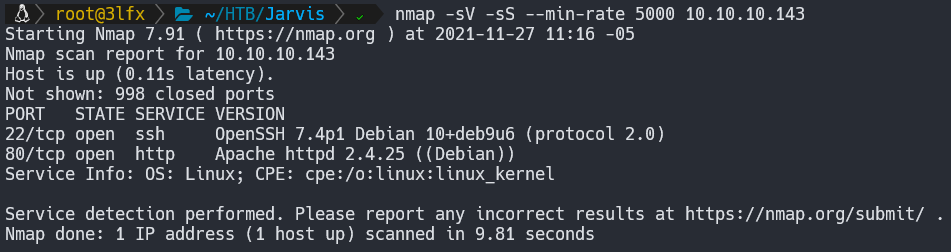
\includegraphics[width=1\textwidth]{imagenes/nmap_jarvis.png} \par \vspace{0.1cm}
            \caption{Escaneo de puertos Jarvis} 
        \end{figure}
    \subsubsection{Análisis de vulnerabilidades y debilidades}
        